% Sample LaTeX file for creating a paper in the Morgan Kaufmannn two
% column, 8 1/2 by 11 inch proceedings format.

\documentclass[letterpaper]{article}
\usepackage{uai2019}
\usepackage[margin=1in]{geometry}

% Set the typeface to Times Roman
\usepackage{times}

\usepackage{algorithm,algorithmic}
\newcommand{\theHalgorithm}{\arabic{algorithm}}

\usepackage{microtype}
\usepackage{graphicx}
\usepackage{subfigure}
\usepackage{booktabs} % for professional tables

\usepackage{natbib}

\usepackage{amssymb} %maths
\usepackage{amsmath} %maths
\usepackage{amsthm}
\usepackage{hyperref}
\usepackage[utf8]{inputenc} %useful to type directly diacritic characters
\usepackage[capitalize]{cleveref}
\crefname{prop}{Proposition}{Propositions}
\crefname{thm}{Theorem}{Theorems}
\crefname{lem}{Lemma}{Lemmas}
\crefname{algorithm}{Algorithm}{Algorithms}

\def\rva{{\mathbf{a}}}
\def\rvo{{\mathbf{o}}}
\def\rvr{{\mathbf{r}}}
\def\rvs{{\mathbf{s}}}
\def\rvu{{\mathbf{u}}}
\def\rvw{{\mathbf{w}}}
\def\rvx{{\mathbf{x}}}
\def\rvg{{\mathbf{g}}}
\def\rvo{{\mathbf{o}}}
\def\rvone{{\mathbf{1}}}
\def\rvzero{{\mathbf{0}}}
\def\rvtilder{{\tilde{\mathbf{r}}}}
\def\rvhat{{\hat{\mathbf{r}}}}

\def\rvp{{\mathbf{p}}}

\def\pr{{\text{Pr}}}
\def\r{{\text{R}}}

\def\ucb{{\text{U}}}
\def\lcb{{\text{L}}}

\newtheorem{thm}{Theorem}
\newtheorem{lem}{Lemma}
\newtheorem{defi}{Definition}
\newtheorem{prop}{Proposition}
\newtheorem{remk}{Remark}

\def\rvpi{{\boldsymbol{\pi}}}

\def\rmA{{\mathbf{A}}}
\def\rmD{{\mathbf{D}}}
\def\rmH{{\mathbf{H}}}
\def\rmI{{\mathbf{I}}}
\def\rmW{{\mathbf{W}}}
\def\rmX{{\mathbf{X}}}

\def\sE{{\mathbb{E}}}
\def\sR{{\mathbb{R}}}
\def\sI{{\mathbb{I}}}
\def\sP{{\mathbb{P}}}

\def\gN{{\mathcal{N}}}
\def\gE{{\mathcal{E}}}
\def\gU{{\mathcal{U}}}

\DeclareMathOperator*{\argmax}{arg\,max}
\DeclareMathOperator*{\argmin}{arg\,min}
\DeclareMathOperator*{\probability}{Pr}
\DeclareMathOperator*{\expectation}{\sE}

\title{On Provable Policy Gradient Methods and Optimal Stochastic Bandit Algorithms with Neural Networks}

\author{} % LEAVE BLANK FOR ORIGINAL SUBMISSION.
          % UAI  reviewing is double-blind.

% The author names and affiliations should appear only in the accepted paper.
%
%\author{ {\bf Harry Q.~Bovik\thanks{Footnote for author to give an
%alternate address.}} \\
%Computer Science Dept. \\
%Cranberry University\\
%Pittsburgh, PA 15213 \\
%\And
%{\bf Coauthor}  \\
%Affiliation          \\
%Address \\
%\And
%{\bf Coauthor}   \\
%Affiliation \\
%Address    \\
%(if needed)\\
%}

\begin{document}

\maketitle

\begin{abstract}
We propose a deep reinforcement learning algorithm that achieves nearly optimal finite time regret in the stochastic bandit setting. In the proposed approach, the agent maintains its action selection strategy as a parametric model. After sufficient exploration, a neural network is trained to minimize an empirical value estimate using gradient updates. The policy is obtained from the exponentiation of the learned logits. While this method differs from standard bandit algorithms, which directly utilize statistics from sampled data, we show that its finite time regret is nearly optimal up to log and constant factors. These results can be generalized to episodic MDPs and the state dependent bandit cases.
\end{abstract}

\section{Introduction}
\label{sec:introduction}

Traditional reinforcement learning (RL) algorithms usually enjoy favorable theoretical guarantees under the the tabular cases of the bandit settings and the Markov decision process (MDP) setting \citep{sutton2018reinforcement}.
%In the traditional RL field, without the DL function approximations, there are many algorithms enjoying favorable theoretical guarantees, under the the tabular cases of the bandit settings and the Markov decision process (MDP) setting \citep{sutton2018reinforcement}. 
For example, (nearly) optimal algorithms have been discovered to achieve finite time regret upper bounds under the stochastic and adversarial bandit settings \citep{bubeck2012regret}. Q-learning is proved to be efficient in an episodic MDP setting \cite{jin2018q}. With linear and smooth function approximations, the Gradient Temporal Difference method and its variants have also been proved to converge to the fixed points of the projected Bellman operators, though the performance of the fixed-point policies can be arbitrarily bad, without imposing any further constraints on the function approximation classes \citep{sutton2009fast,sutton2009convergent,bhatnagar2009convergent}.

In recent years, deep reinforcement learning (DRL) methods have further improved traditional RL methods in practice and achieved a number of great successes, including professional level game players in Go \citep{silver2016masteringA,silver2017masteringB}, Atari \citep{mnih2015human}, Poker \citep{moravvcik2017deepstack}, and robotic controls \citep{lillicrap2015continuous,levine2016end}.
In particular, DRL methods optimize RL objectives during learning while employing deep neural networks as function approximations, thus combine the rich representation power of neural networks and the effective learning strategies from RL \citep{sutton2018reinforcement}. 
However, also mainly due to the complex behavior of neural networks, theoretical analyses of DRL methods become extremely difficult.
Existing analyses in the literature usually contain various unverifiable assumptions. \citep{krishnamurthy2016pac} assumes that the global optimal policy is contained in the parametric function class. \citep{dai2018sbeed} assumes having knowledge of the function approximation errors, which cannot be obtained in practice.
Moreover, these works do not particularly focus on neural networks. Although their results can be generally applied to DRL methods, their analyses do not reflect the improvement by using neural networks as function approximations. 

In this paper, we take one step further to theoretically understand the behavior of DRL methods. In particular, we propose two DRL methods, one value based and the other policy based. Our methods, while not exactly the same as popular DRL methods in the literature, catch the essences of value based and policy based DRL methods. To summarize, our contributions are as follows.
\begin{itemize}
	\item We propose a policy based RL method, Policy Gradient with Uniform Exploration (PGE), that is similar to the vanilla policy gradient method, but mixed with an uniform exploration and a momentum on the rewards. We prove that PGE, with over-parametrized neural network as its policy network, enjoys a sub-linear finite time convergence rate under the stochastic bandit setting.
	\item We further propose a value based RL method, Logit Learning with $\varepsilon$-Greedy Exploration (LLE), which, again with over-parametrized neural network as its value network, achieves a nearly optimal regret under the stochastic bandit setting. This algorithm learns value based objectives using the gradient descent. 
	\item We discuss how our results can be easily generalized to many other reinforcement learning settings, such as the state dependent stochastic bandit settings and episodic MDPs.
\end{itemize}

To our best knowledge, this paper is the first result in the literature on the optimization theory of RL methods with neural networks as function approximations. Our results can be seen as an initial step toward understanding the globally convergence for the popular RL methods (the value based learning, and the policy gradient here) with non-linear neural network function approximations, such as Deep Q-Network \cite{mnih2015human}, Asynchronous Actor-Critic Agents \citep{mnih2016asynchronous}, Path Consistency Learning \citep{nachum2017bridging}, and Relative Entropy Policy Search \citep{peters2010relative}, combining with more practical function approximations and training procedures.

Finally, let us comment on the technique side of our results. 
Our results are inspired by the recent progresses on over-parametrized neural networks for supervised learning (regression and classification) \citep{li2018learning,du2018gradientA,du2018gradientB,allen2018convergenceA,allen2018convergenceB}. 
However, because of the different learning settings between supervised learning and reinforcement learning, many challenges still persist. 
One standard challenge is the balance between exploration and exploitation in the RL/bandits problems.
Such balance in our problem becomes more complex, compared to that in the traditional multi-arm bandit setting, as the update of model is performed by gradient descent on the parameters.
The information gained from one arm will affect the evaluation of the other arms through the parameters of the network, which may help or hurdle the exploration of other arms.
Another challenge is that there is no true label provided by the environment, so the learning objective itself needs to be estimated from the collected data.
We propose to use the empirical average rewards instead of a single reward on the current step for the learning objective. 
Note that even so we still do NOT have an accurate estimate on the rewards.
To see that, as we hope that our policy can achieve a sub-linear (or nearly optimal) regret rate, only a limited budget (sub-linear or $O(\ln T )$) is allowed for the sub-optimal arms. Thus, as a sharp contrast to supervised learning with i.i.d. samples, we do NOT have enough samples from the sub-optimal arms for accurate estimates.  


%In the DL field, the well known situation is that the theoretical understanding is far behind with the practical applications \citep{goodfellow2016deep,zhang2016understanding}. Fortunately, there are still continuous progresses in several aspects, including expressiveness \citep{cybenko1989approximation,raghu2017expressive}, optimization \citep{kawaguchi2016deep,li2017convergence,li2018learning,du2018gradientA,du2018gradientB,allen2018convergenceA,allen2018convergenceB}, and generalization \cite{neyshabur2017exploring,allen2018learning} of the DL theory. 
%In particular, very recently, it has been discovered that, for over-parameterized neural networks, i.e., given that the numbers of parameters in the hidden layers are quite large (usually polynomial over the number of training data points), zero training loss can be achieved using the gradient descent and stochastic gradient descent methods, under the supervised learning (regression and classification) settings \citep{li2018learning,du2018gradientA,du2018gradientB,allen2018convergenceA,allen2018convergenceB}. With some additional structured data distribution assumptions, the convergent training loss can be generalized to the testing loss, endowing the learned neural network provable generalization abilities \citep{li2018learning,allen2018learning}.

%However, the recent progresses of the DL theory was developed under the supervised learning settings, which makes it not directly applicable in the RL settings, due to the significant differences between the RL and the supervised learning: (a) when learning RL agents, there is no true label provided by the environment, so the learning objective itself needs to be estimated from the collected data, which makes the RL problems more difficult than optimization problems in the supervised learning; (b) the interaction between the  agent and the environment will also incur losses during learning, which makes the principled ways of exploration matter.

%In this paper, based on the recent work in the optimization theory of over-parameterized neural networks, we take one step forward to theoretically understanding the DRL methods. In particular, our contributions are as follows.
%\begin{itemize}
   % \item We propose Logit Learning with $\varepsilon$-Greedy Exploration, which achieves optimal regret under the stochastic bandit setting. The algorithms learn value based objectives using the gradient descent, with value functions parameterized by neural networks. The results can be generalized to the state dependent stochastic bandit settings, and the episodic MDP settings.
    %\item We prove that the widely used policy gradient methods with uniform exploration also enjoys sublinear finite time regret under the stochastic bandit setting.
%\end{itemize}



The rest of the paper is organized as follows. \cref{subsec:notations} presents the notations.   \cref{sec:background} introduces the background, settings and the network structures. \cref{sec:policy_gradient} proposes the policy gradient algorithm. \cref{sec:logit_learning} proposes the logit learning algorithm. \cref{sec:general_settings} briefly shows the results in several more general settings. \cref{sec:future_work} discusses some open problems and future work. \cref{sec:conclusions} comes to our conclusions. All the formal proofs are deferred to the appendix due to the space limit.

\subsection{Notations}
\label{subsec:notations}
We use bold lowercase letters to refer to vectors, such as $\rvr$, and bold capital letters to refer to matrices, like $\rmW$. Non-bold lowercase letters are scalars. For example, $u_{i,r} \in \sR$ is the $r$th component of vector $\rvu_i \in \sR^m$. $\rvone$ means an all-one vector, and $\rmI$ refers to an identity matrix, with dimensions depend on the contexts. We also denote $[n] \triangleq \left\{ 1,2, \dots, n \right\}$. 

In the sequel, $n$ is the total number of states, and $h$ is the total number of actions that can be taken at each state.
Also, for $i\in[n]$, let $\rvr_i \in \sR^h$ be the true mean reward vector at state $\rvs_i$. $\rvpi_i^* = \argmax_{\rvpi \in \Delta^{h}}{\left\{ \rvpi^\top \rvr_i \right\}}$ is the optimal policy at state $\rvs_i$. Given a sequence of  stochastic policies $\bf{\Pi} \triangleq \left[ \rvpi_1, \rvpi_2, \dots, \rvpi_n \right] \in {\sR}^{h \times n}$, the expected (mean) loss is defined as,
\begin{equation}
\label{eq:expected_loss}
\begin{split}
\frac{1}{n} \cdot \sum\limits_{i=1}^{n}{ \left( {\rvpi_i^*}^\top \rvr_i - \rvpi_i^\top \rvr_i \right) }.
\end{split}
\end{equation}

We use two-layer fully connected neural networks with ReLU activation as our value function and policy function approximations, as shown in \cref{fig:nn_policy_value}. 
%The structure of the value network and the policy network  is a 2-layers fully connected neural network with ReLU activation, 
Each neural network takes the state $\rvs \in \sR^d$ as its input. 
For the first layer, we use $\rvs_i \in \sR^d$ for $i \in [n]$ refers to the feature vector of the $i$th state, $\rvw_r \in \sR^d$ for $r \in [m]$ to a weight vector in the first hidden layer, and $u_{i,r} \triangleq \rvw_r^\top \rvs_i$ to the $r$th node value of the first hidden layer.
Let $\rmW^\top \triangleq \left[ \rvw_1, \rvw_2, \dots, \rvw_m \right] \in \sR^{d \times m}$ be the weight matrix of the first hidden layer, thus the hidden layer is $\rvu = \rmW\rvs\in\sR^m$.

Similarly let $\rva_k \in \sR^m$ for $k \in [h]$ be a weight vector in the second hidden layer, and $o_{i,k} \triangleq \sum_{r=1}^{m}{a_{k,r} \cdot \sigma\left( u_{i,r} \right)}$ be the logit of the $k$th action for state $\rvs_i$, where $\sigma(\cdot) = \max\left\{ \cdot, 0 \right\}$ is the ReLU activation function. 
Let $\rmA^\top \triangleq \left[ \rva_1, \rva_2, \dots, \rva_h \right] \in \sR^{m \times h}$ be the weight matrix of the second hidden layer, then the logit output $\rvo = \rmA\sigma\left( \rvu\right) \in \sR^h$.

Lastly, the policy network differs the value network with one additional softmax transform layer in order to output probability distributions, where $\rvpi \triangleq f\left( \rvo \right) = f\left( \rmA \sigma\left( \rmW \rvs \right) \right)$ and $f$ is the softmax function: $f\left( o_{i,k} \right) = \exp\left\{ o_{i,k} \right\} \,/\, \sum_{k^\prime = 1}^{h}{\exp\left\{ o_{i,k^\prime} \right\}}$.

\section{Background}
\label{sec:background}

\begin{figure}[t]
	%\vskip 0.2in
	\begin{center}
		\centerline{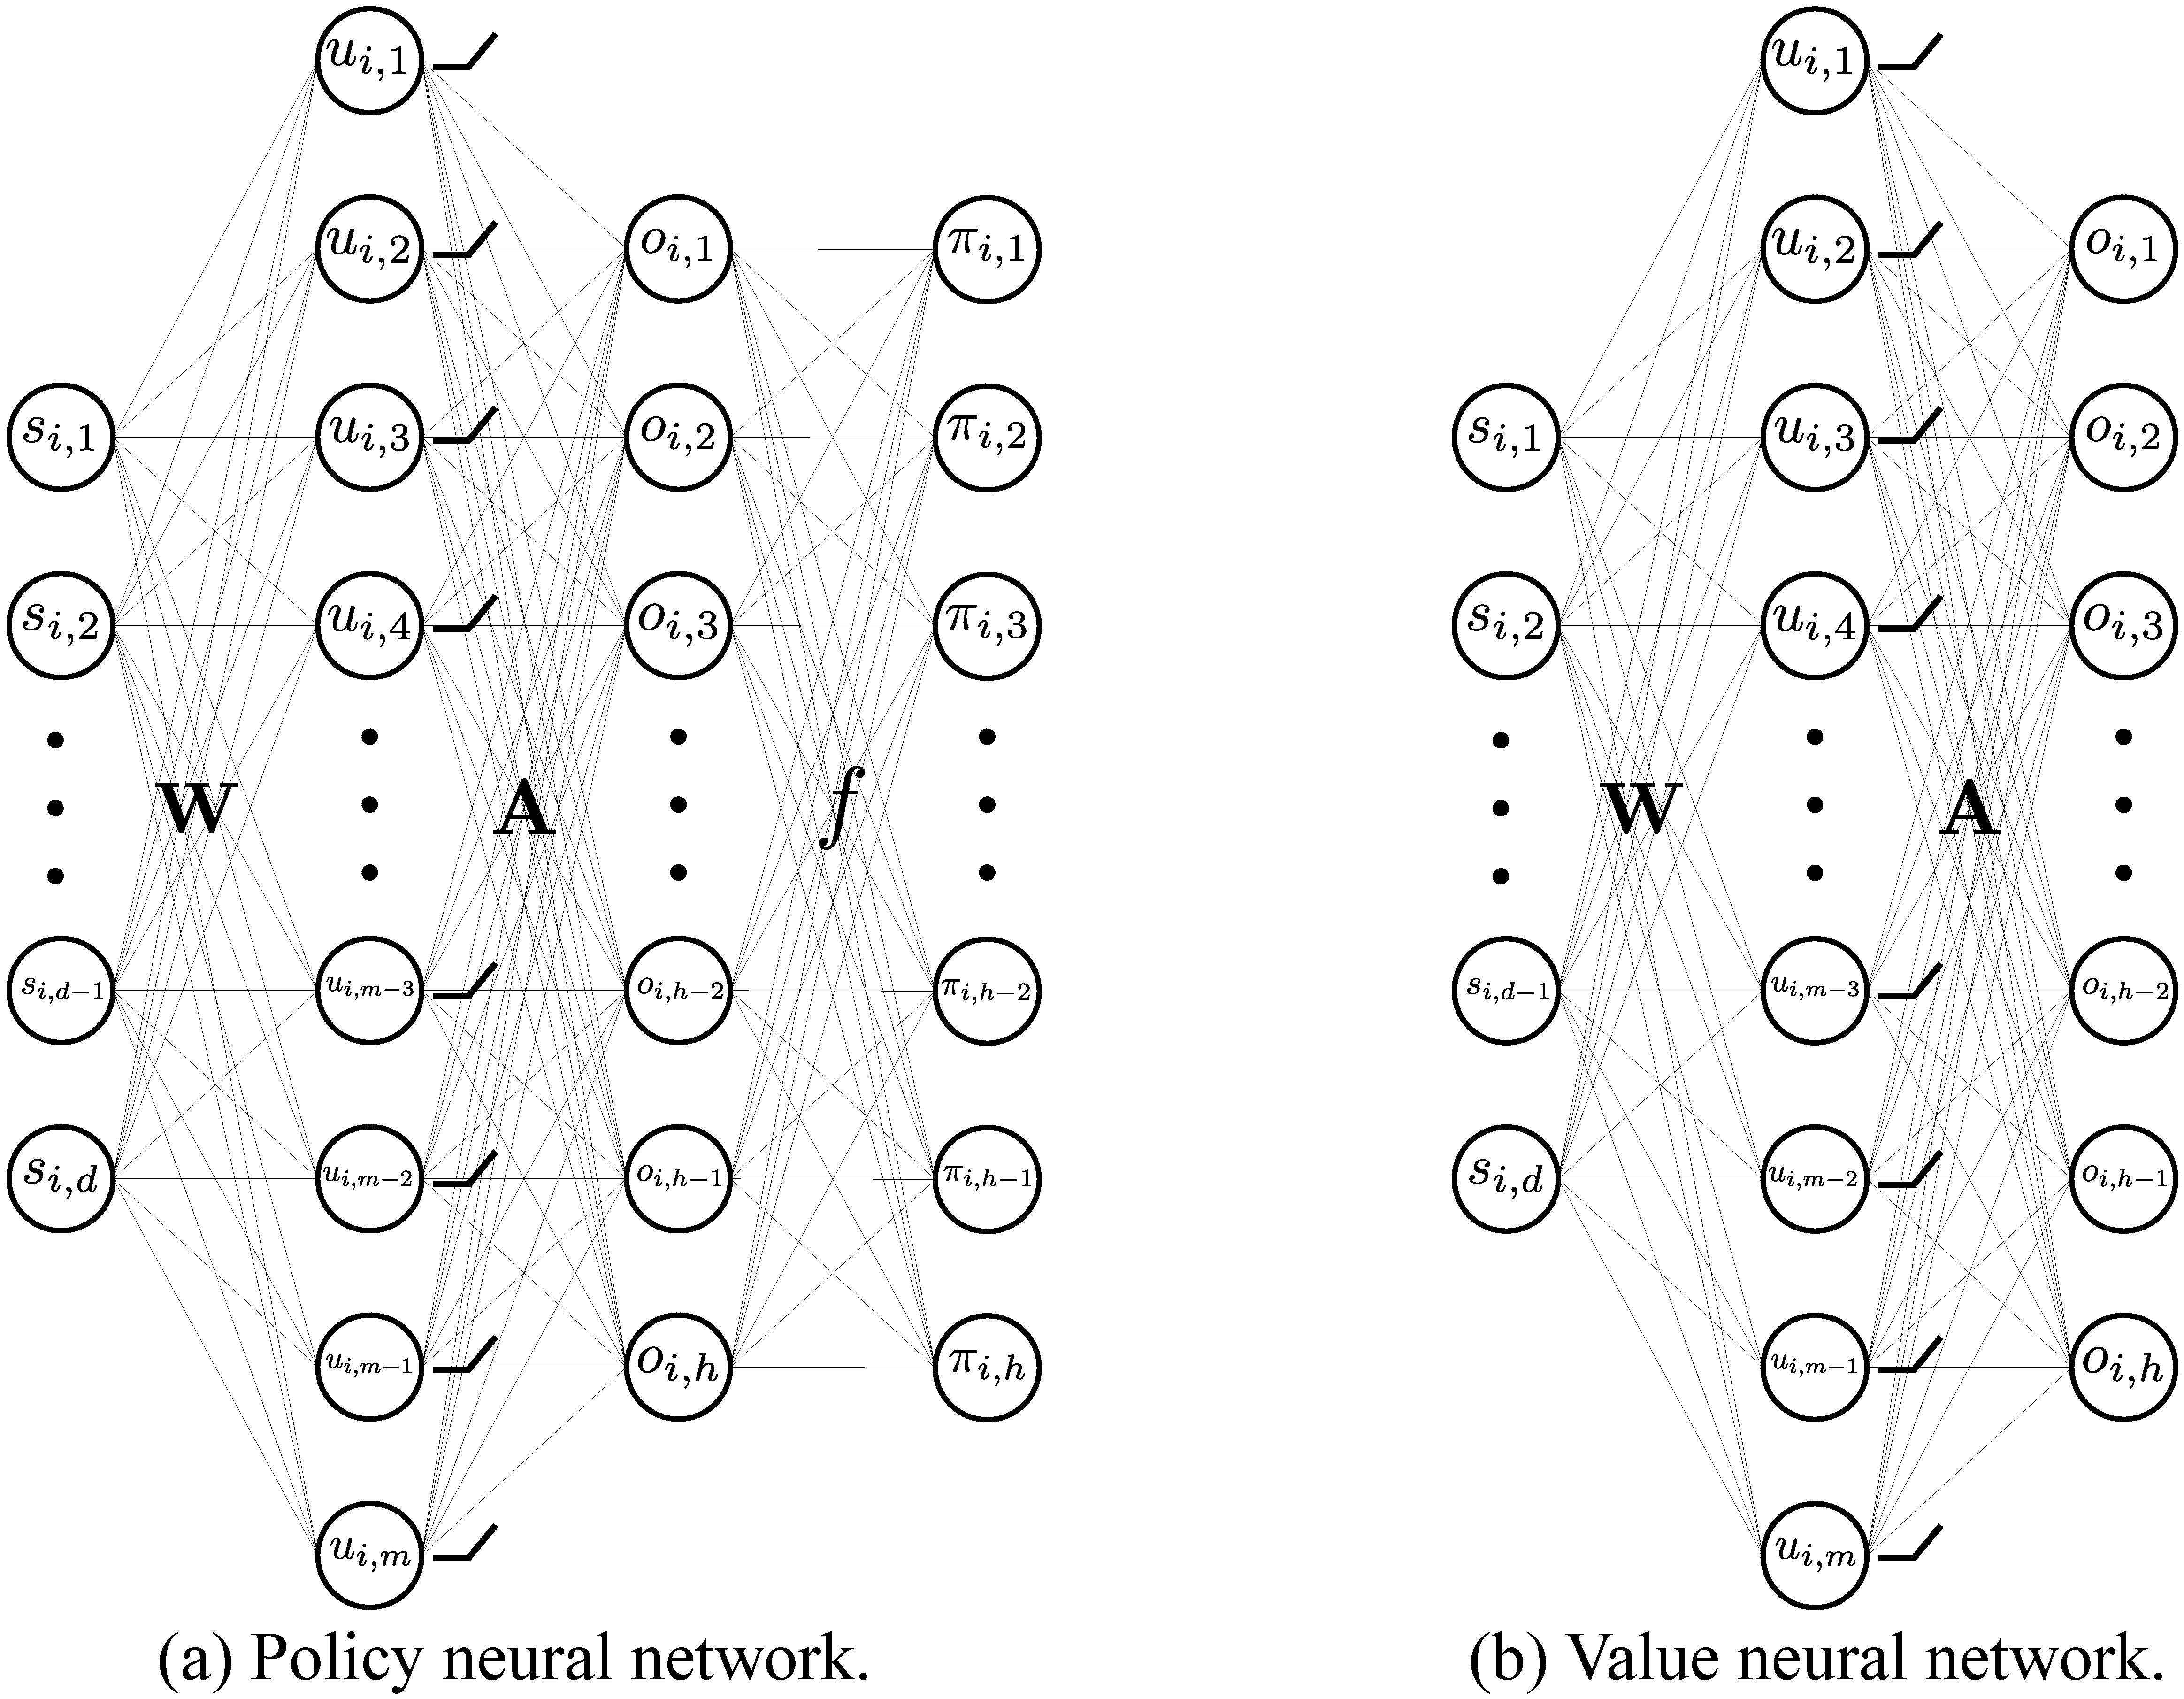
\includegraphics[width=0.7\columnwidth]{nn_policy_value_vertical.pdf}}
		\caption{The structure of the policy neural network and the value neural network.}
		\label{fig:nn_policy_value}
	\end{center}
	\vskip -0.2in
\end{figure}

We focus on the stochastic bandit setting in this paper where the policy or the values of the actions are represented using a 2-layers neural networks.  
However, our results can be easily generalized to many other reinforcement learning settings, e.g. state dependent stochastic bandit settings and episodic MDP settings.

\subsection{Stochastic Bandit Settings}
\label{subsec:settings}

One can think of that the standard stochastic bandit setting has only 1 state.  
At each time step $t$, the agent takes an action $A_t \in [h]$ according to its own strategies $\rvpi_t$, and then it observes a random reward $R\left(A_t\right) \in \sR$, where the mean value of $R\left(A_t\right)$ is $r\left(A_t\right)$. 
The agent then improves its action selection strategies. 
After such $T$ time steps, the performance of the agent's strategy is measured by the (expected) regret,
\begin{equation}
\label{eq:expected_regret}
R_T = \sum\limits_{t=0}^{T-1}{{\rvpi^*}^\top \rvr} - \sE \left[ \sum\limits_{t=0}^{T-1}{  r\left(A_t\right)  } \right] 
%= \sum\limits_{t=0}^{T-1}{{\rvpi^*}^\top \rvr} - \sum\limits_{t=0}^{T-1}{ \sE \left[ r\left(A_t\right) \right] },
\end{equation}
where the expectation is over the randomness of action selection, if the agent is using some stochastic strategies.
Obviously, $\rvpi^*$ is a one-hot vector and by standard calculation, one can show that
\[
R_T = \sum_{t=0}^{T-1} \sum_a \pi_t(a) \Delta(a),
\]
where $\Delta(a) = \max_b r(b)- r(a)$, $r(a)$ is the expected reward of the action $a$.

%\subsubsection{Episodic Markov decision process (MDP) (maybe remove this section)}
%The episodic MDP setting recovers the bandit setting as a special case. The environment randomly select a starting state $\rvs_i^0 \in \sR^d$. At each time step $t$, the agent takes one action $A_t \in [h]$ according to some strategies, and then it observes a reward $R_{i, A_t} \in \sR$ and next state $S_{t+1} \sim \sP\left( \cdot \middle| S_t, A_t \right)$, where $\sP$ is the transition probability matrix and it is unknown to the agent. After such $H$ steps, the agent observes an ending state $S_H$, and the current trajectory terminates. At the next time step, the agent will observe a new starting state $\rvs_i^0$ randomly generated by the environment. Since we use policy gradient method (no value learning), the agent updates its neural network policy weights using the cumulative reward collected after each single trajectory terminates.

%We mainly focus on the standard stochastic bandit setting with $n = 1$, i.e., there is only one state $\rvs_i$. At each time step $t$, the agent takes an action $A_t \in [h]$ according to its own strategies, and then it observes a random reward $R_{i, A_t} \in \sR$, where the mean value of $R_{i, A_t}$ is $r_{i, A_t}$. The agent then uses the reward to improve its action selection strategies. After such $T$ time steps, the performance of the agent's strategy is measured by the (expected) regret,
%\begin{equation}
%\label{eq:expected_regret}
%    \sum\limits_{t=0}^{T-1}{{\rvpi_i^*}^\top \rvr_i} - \sE \left[ \sum\limits_{t=0}^{T-1}{  r_{i, A_t}  } \right] = \sum\limits_{t=0}^{T-1}{{\rvpi_i^*}^\top \rvr_i} - \sum\limits_{t=0}^{T-1}{ \sE \left[ r_{i, A_t} \right] },
%\end{equation}
%where the expectation is over the randomness of action selection, if the agent is using some stochastic strategies.

\subsection{Neural Network Value Function Approximation and Policy}
\label{subsec:nn_value_policy}
The structure of the value network and the policy network  is a 2-layers fully connected neural network with ReLU activation, as shown in \cref{fig:nn_policy_value}. 
Each neural network takes the state $\rvs \in \sR^d$ as its input, where without loss of generality we assume that $\left\| \rvs \right\|_2 = 1$.
The hidden layer of both networks are denoted by $\rvu \triangleq \rmW\rvs\in\sR^m$, and the logit output $\rvo \triangleq \rmA\sigma\left( \rvu\right) \in \sR^h$, where $\sigma$ is element-wise ReLU activation function. The policy network differs the value network with one additional softmax transform layer in order to output probability distributions, where $\rvpi \triangleq f\left( \rvo \right) = f\left( \rmA \sigma\left( \rmW \rvs \right) \right)$, and $f$ is the softmax function. 

%Both the value and the policy neural networks take the state feature  $\rvs_i \in \sR^d$ as the input. Then the networks calculate the hidden node value vector by $u_{i,r} \triangleq \rvw_r^\top \rvs_i$, $\forall r \in [m]$. The logit vector is then calculated by $o_{i,k} \triangleq \rva_k^\top \sigma\left( \rvu_i \right)$, $\forall k \in [h]$, where $\sigma$ is element-wise ReLU activation function. The value neural network outputs the logit vector $\rvo_i$. While the policy neural network output probability is the softmax transform of the logit vector, i.e., $\rvpi_i \triangleq f\left( \rvo_i \right) = f\left( \rmA \sigma\left( \rmW \rvs_i \right) \right)$. 

%The policy neural network defines a family of policies $\rvpi_i \left( \rmW \right)$ parameterized by $\rmW \in \sR^{m \times d}$ given any state $\rvs_i$. Let $\rvpi_i = \rvpi_i \left( \rmW \right)$, the expected loss of the policy neural network can be calculated according to \cref{eq:expected_loss}.

\paragraph{Initialization of the matrix $\rmA$.} 
As can be seen later, our algorithm random initializes the weight matrix $\rmA$ and fixes it during learning. 
This is a common strategy when using over-parametrization neural networks, e.g. see \citep{li2018learning,du2018gradientA,du2018gradientB,allen2018convergenceA,allen2018convergenceB}, and it has been empirically verified that there is no impact on the performance of trained neural networks \citep{hoffer2018fix}.
In this paper, each element in $\rmA$ is initialized by $a_{k,r} \sim \gU\left\{-1, +1\right\}$, $a_{k,r}$. Some other initializations like $\rva_k \sim \gN(0, \rmI)$ will also work. Thus in the rest of the paper, we denote the policy $\rvpi$ by $\rvpi(\rmW_t)$ to emphasize its parametrization by $\rmW$ at time step $t$. 

\paragraph{Multi-layered neural networks.} We would like to point that our algorithms and results can be easily extended to general value functions and policies parameterized by multi-layered neural networks \citep{allen2018convergenceA,allen2018convergenceB,du2018gradientA}. For the sake of simplicity and conciseness, we only focus on two-layers neural networks in the paper.

%Although there is only one state, i.e., $n = 1$, and $i$ can be omitted without ambiguity, we choose to keep the subscript $i$ here to make the generalization from the standard bandit setting to the many state dependent setting smoother, and our algorithms work for general $n > 1$. For simplicity, we assume $\left\| \rvs_{i} \right\|_2 = 1$, $\forall i \in [n]$.

%In the case of $n > 1$, for each state $\rvs_i$, there is a state dependent policy $\rvpi_i$. And the agent's goal is to learn totally $n$ policies using only one neural network. We assume $\left\| \rvs_{i} -  \rvs_{j} \right\|_2 \ge \delta > 0 , \ \forall i \not= j$, i.e., no duplicated data, and $\left\| \rvs_{i} \right\|_2 = 1, \ \forall i \in [n]$.


\section{Theoretical Analysis}
\label{sec:theoretical_analysis}

\subsection{Main Results}
\label{subsec:main_results}

We first present the main results in the bandit settings, as shown in \cref{thm:main_result}, and then show the detailed proof ideas and  intuitions.

\begin{thm}
\label{thm:main_result}
    Given a two layer NN policy $\rvpi_i$, with number of parameters $m \in \Theta\left( \frac{n^{10}}{c^4 \delta^4 \varepsilon^2} \right)$, $\eta = \frac{1}{4 h m}$, the expected regret of \cref{alg:policy_gradient_uniform_exploration} satisfies,
\begin{equation*}
\begin{split}
    &\sum\limits_{t=0}^{T-1}{ {\rvpi_i^*}^\top \rvr_i } - \sum\limits_{t=0}^{T-1}{ \sE \left[ r_{i, A_t} \right] } \\
    &\le \frac{8 h}{c} \cdot T^{\frac{2}{3}} + 3 \log{h} \cdot T^{\frac{2}{3}} \left(\log{T}\right)^{\frac{1}{3}}
\end{split}
\end{equation*}
\end{thm}
\begin{proof}
According to \cref{alg:policy_gradient_uniform_exploration}, the uniform policy and $\rvpi_i\left( \rmW(t) \right)$ are used to sample actions int the two phases. Therefore the regret is divided into two parts.
\begin{equation}
\small
\label{eq:total_regret_decomposition}
\begin{split}
    &\sum\limits_{t=0}^{T-1}{ {\rvpi_i^*}^\top \rvr_i } - \sum\limits_{t=0}^{T-1}{ \sE \left[ r_{i, A_t} \right] } = \sum\limits_{t=0}^{T^{\frac{2}{3} + \beta} - 1}{ \left[ {\rvpi_i^*}^\top \rvr_i  \right]} \\
    &\quad - \sum\limits_{t=0}^{T^{\frac{2}{3} + \beta} - 1}{ \expectation\limits_{A_t \sim \gU\left[h\right]}{ \left[ r_{i, A_t} \right] }} + \sum\limits_{t=T^{\frac{2}{3} + \beta}}^{T-1}{ {\rvpi_i^*}^\top \rvr_i } \\
    &\quad - \sum\limits_{t=T^{\frac{2}{3} + \beta}}^{T-1}{ \rvpi_i\left( \rmW(t) \right)^\top \rvr_i } \\
    &\le \sum\limits_{t=0}^{T^{\frac{2}{3} + \beta} - 1}{1} + \sum\limits_{t=T^{\frac{2}{3} + \beta}}^{T-1}{ {\rvpi_i^*}^\top \rvr_i } - \sum\limits_{t=T^{\frac{2}{3} + \beta}}^{T-1}{ \rvpi_i\left( \rmW(t) \right)^\top \rvr_i } \\
    &= T^{\frac{2}{3} + \beta} + \sum\limits_{t=T^{\frac{2}{3} + \beta}}^{T-1}{ {\rvpi_i^*}^\top \rvr_i } - \sum\limits_{t=T^{\frac{2}{3} + \beta}}^{T-1}{ \rvpi_i\left( \rmW(t) \right)^\top \rvr_i }.
\end{split}
\end{equation}
Denote $\rvpi_i^*\left(t\right) \triangleq \argmax\limits_{\rvpi \in \Delta^{h-1}}{\left\{ \rvpi^\top \hat{\rvr}_i\left(t\right)\right\}}$. The last two terms can be decomposed as,
\begin{equation}
\small
\label{eq:playing_learning_phase_regret_decomposition}
\begin{split}
    &\sum\limits_{t=T^{\frac{2}{3} + \beta}}^{T-1}{ \left( {\rvpi_i^*} - \rvpi_i\left( \rmW(t) \right) \right)^\top \rvr_i } \\
    &= \sum\limits_{t=T^{\frac{2}{3} + \beta}}^{T-1}{ \left( {\rvpi_i^*\left(t\right)} - \rvpi_i\left( \rmW(t) \right) \right)^\top \hat{\rvr}_i\left(t\right) } \\
    &\quad - \sum\limits_{t=T^{\frac{2}{3} + \beta}}^{T-1}{ \left( {\rvpi_i^*\left(t\right)} - {\rvpi_i^*} \right)^\top \hat{\rvr}_i\left(t\right) } \\
    &\quad + \sum\limits_{t=T^{\frac{2}{3} + \beta}}^{T-1}{  \left( \rvpi_i\left( \rmW(t) \right) - {\rvpi_i^*}\right)^\top \left(  \hat{\rvr}_i\left(t\right) - \rvr_i \right) } \\
    &\le \sum\limits_{t=T^{\frac{2}{3} + \beta}}^{T-1}{ \left( {\rvpi_i^*\left(t\right)} - \rvpi_i\left( \rmW(t) \right) \right)^\top \hat{\rvr}_i\left(t\right) } \\
    &\quad + \sum\limits_{t=T^{\frac{2}{3} + \beta}}^{T-1}{  \left\| \rvpi_i\left( \rmW(t) \right) - \rvpi_i^* \right\|_1 \cdot \left\| \hat{\rvr}_i\left(t\right) - \rvr_i \right\|_\infty } \\
    &\le \sum\limits_{t=T^{\frac{2}{3} + \beta}}^{T-1}{ \left( {\rvpi_i^*\left(t\right)} - \rvpi_i\left( \rmW(t) \right) \right)^\top \hat{\rvr}_i\left(t\right) } \\
    &\quad + 4 T \exp\left\{ - \frac{2}{h} \cdot  T^{3\beta} \right\} + 2 T^{\frac{2}{3} + \beta},
\end{split}
\end{equation}
by the definition of $\rvpi_i^*\left(t\right)$, H{\"o}lder's inequality, and \cref{thm:loss_estimation_hoeffding}. Denote $\omega_t \triangleq \left( {\rvpi_i^*\left(t\right)} - \rvpi_i\left( \rmW(t) \right) \right)^\top \hat{\rvr}_i\left(t\right)$.
\begin{equation}
\label{eq:dynamic_regret_decomposition}
\begin{split}
    \omega_t &= {\rvpi_i^*\left(t\right)}^\top \left( \hat{\rvr}_i\left(t\right) - \hat{\rvr}_i\left(t-1\right)\right) \\
    &\quad + \left( {\rvpi_i^*\left(t\right)} - {\rvpi_i^*\left(t-1\right)} \right)^\top \hat{\rvr}_i\left(t-1\right) \\
    &\quad + \left( {\rvpi_i^*\left(t-1\right)} - \rvpi_i\left( \rmW(t-1) \right) \right)^\top \hat{\rvr}_i\left(t-1\right) \\
    &\quad + \left(  \rvpi_i\left( \rmW(t-1) \right) - \rvpi_i\left( \rmW(t) \right) 
    \right)^\top \hat{\rvr}_i\left(t-1\right) \\
    &\quad + \rvpi_i\left( \rmW(t) \right)^\top \left( \hat{\rvr}_i\left(t-1\right) - \hat{\rvr}_i\left(t\right)  \right).
\end{split}
\end{equation}
We upper bound each term in the right hand side. Firstly,
\begin{equation*}
\tiny
\begin{split}
    &{\rvpi_i^*\left(t\right)}^\top \left( \hat{\rvr}_i\left(t\right) - \hat{\rvr}_i\left(t-1\right)\right) \\
    &= {\rvpi_{i, A_{t-1}}^*\left(t\right)} \left[ \frac{\sum\limits_{s=0}^{n_{i, A_{t-1}}\left(t\right)-1}{R_{i, A_{t-1}}\left(s\right)}}{n_{i, A_{t-1}}\left(t\right)} - \frac{\sum\limits_{s=0}^{n_{i, A_{t-1}}\left(t-1\right)-1}{R_{i, A_{t-1}}\left(s\right)}}{n_{i, A_{t-1}}\left(t-1\right)} \right] \\
    &= \frac{{\rvpi_{i, A_{t-1}}^*\left(t\right)}}{n_{i, A_{t-1}}\left(t\right)} \left( R_{i, A_{t-1}}\left( n_{i, A_{t-1}}\left(t\right) -1 \right) - \hat{r}_{i, A_{t-1}}\left(t-1\right) \right) \\
    &\le \frac{1}{n_{i, A_{t-1}}\left(t\right)} \le \frac{h}{T^{\frac{2}{3} + \beta}},
\end{split}
\end{equation*}
by $n_{i, A_{t-1}}\left(t\right) = n_{i, A_{t-1}}\left(t-1\right) + 1$, and $n_{i, A_{t-1}}\left(t\right) \ge \frac{T^{\frac{2}{3} + \beta}}{h}$, $\forall t \ge T^{\frac{2}{3} + \beta}$. By the definition of ${\rvpi_i^*\left(t-1\right)}$,
\begin{equation*}
    \left( {\rvpi_i^*\left(t\right)} - {\rvpi_i^*\left(t-1\right)} \right)^\top \hat{\rvr}_i\left(t-1\right) \le 0.
\end{equation*}
Note that according to the definition of $\omega_t$,
\begin{equation*}
    \left( {\rvpi_i^*\left(t-1\right)} - \rvpi_i\left( \rmW(t-1) \right) \right)^\top \hat{\rvr}_i\left(t-1\right) = \omega_{t-1}.
\end{equation*}
By \cref{lem:parameter_smoothness}, $\eta = \frac{1}{4hm}$, and \cref{lem:gradient_lower_bound},
\begin{equation*}
\begin{split}
    &\left(  \rvpi_i\left( \rmW(t-1) \right) - \rvpi_i\left( \rmW(t) \right) 
    \right)^\top \hat{\rvr}_i\left(t-1\right) \\
    &\le - \frac{1}{8 h m} \left\| \frac{d \rvpi_i\left( \rmW(t-1) \right)^\top \hat{\rvr}_i\left(t-1\right)}{d \rmW(t-1)} \right\|_F^2 \\
    &= - \frac{1}{8 h m} \sum\limits_{r=1}^{m}{ \left\| \frac{d \rvpi_i\left( \rmW(t-1) \right)^\top \hat{\rvr}_i\left(t-1\right)}{d \rvw_r(t-1)} \right\|_2^2 } \\
    &\le - \frac{\delta^2 c^2}{8 h n^4} \left[ \left( {\rvpi_i^*\left(t-1\right)} - \rvpi_i\left( \rmW(t-1) \right) \right)^\top \hat{\rvr}_i\left(t-1\right)  \right]^2 \\
    &= - \frac{\delta^2 c^2}{8 h n^4} \cdot \omega_{t-1}^2.
\end{split}
\end{equation*}
Using similar arguments,
\begin{equation*}
    \rvpi_i\left( \rmW(t) \right)^\top \left( \hat{\rvr}_i\left(t-1\right) - \hat{\rvr}_i\left(t\right)  \right) \le \frac{h}{T^{\frac{2}{3} + \beta}}.
\end{equation*}
Plugging the above upper bounds into \cref{eq:dynamic_regret_decomposition},
\begin{equation*}
    \omega_t \le \omega_{t-1} - \frac{\delta^2 c^2}{8 h n^4} \cdot \omega_{t-1}^2 + \frac{2h}{T^{\frac{2}{3} + \beta}}
\end{equation*}
Rearranging and summing up from $T^{\frac{2}{3} + \beta} + 1$ to $T$,
\begin{equation*}
\begin{split}
    \sum\limits_{t=T^{\frac{2}{3}+ \beta}+1}^{T}{\omega_{t-1}^2} &\le \frac{8 h n^4}{\delta^2 c^2} \sum\limits_{t=T^{\frac{2}{3}+ \beta}+1}^{T} { \left[ \omega_{t-1} - \omega_t + \frac{2h}{T^{\frac{2}{3} + \beta}} \right] } \\
    &\le \frac{16 h^2 n^4}{\delta^2 c^2} \cdot T^{\frac{1}{3} - \beta}.
\end{split}
\end{equation*}
By the Root-Mean Square-Arithmetic Mean inequality,
\begin{equation*}
\begin{split}
    \sum\limits_{t=T^{\frac{2}{3}+ \beta}}^{T-1}{\omega_{t}} &\le \sqrt{\left(T  - T^{\frac{2}{3}+ \beta} \right) \sum\limits_{t=T^{\frac{2}{3}+ \beta}+1}^{T}{\omega_{t-1}^2}} \\
    &\le \frac{4 h n^2}{\delta c} \cdot T^{\frac{2}{3} - \frac{\beta}{2}}.
\end{split}
\end{equation*}
Combining the above with \cref{eq:total_regret_decomposition} and \cref{eq:playing_learning_phase_regret_decomposition},
\begin{equation*}
\begin{split}
    &\sum\limits_{t=0}^{T-1}{ {\rvpi_i^*}^\top \rvr_i } - \sum\limits_{t=0}^{T-1}{ \sE \left[ r_{i, A_t} \right] } \\
    &\le  4 T \exp\left\{ - \frac{2}{h} \cdot  T^{3\beta} \right\} + 3 T^{\frac{2}{3} + \beta} + \frac{4 h n^2}{\delta c} \cdot T^{\frac{2}{3} - \frac{\beta}{2}}
\end{split}
\end{equation*}
Finally, let $\beta = \left( \log{\left(\frac{h}{6}\right) + \log{\log{T}} } \right)/\left(3 \log{T}\right)$, we have $T \exp\left\{ - \frac{2}{h} \cdot  T^{3\beta} \right\} = T^{\frac{2}{3}}$, and $T^{\frac{2}{3} + \beta} = \left( \log{\left(\frac{h}{6}\right)}\right)^{\frac{1}{3}} T^{\frac{2}{3}} \left(\log{T}\right)^{\frac{1}{3}}$.
\end{proof}

\cref{alg:policy_gradient_uniform_exploration} divides $T$ steps into two parts. In the first exploring phase, the agent uniformly samples actions without learning the NN policy. Intuitively, at the beginning, when the loss estimation is very inaccurate, early updating can probably hurt the NN policy.  While in the second playing-learning phase, since the loss estimation is good, the NN policy will keep reducing its surrogate expected loss, which is highly related to its true expected loss, which is identical with the expected regret of this phase.

\subsection{Exploring Phase}
\label{subsec:exploring_phase}

The exploring phase of \cref{alg:policy_gradient_uniform_exploration} provides us good estimations of the true mean loss/reward as follows.
\begin{thm}
\label{thm:loss_estimation_hoeffding}
    In \cref{alg:policy_gradient_uniform_exploration}, $\forall t \ge T^{\frac{2}{3} + \beta}$,
\begin{equation*}
    \left\| \hat{\rvr}_i\left(t\right) - \rvr_i \right\|_\infty \le 2 \exp\left\{ - \frac{2}{h} \cdot  T^{3\beta} \right\} + T^{\beta - \frac{1}{3}}.
\end{equation*}
\end{thm}
\begin{proof}
    At step $t \ge T^{\frac{2}{3} + \beta}$, the $k$th action is sampled $n_{i, k}\left(t\right) \ge \frac{T^{\frac{2}{3} + \beta} }{h}$ times because of the exploring phase, $\forall k \in [h]$. By Hoeffding's inequality, $\forall k \in [h]$,
\begin{equation}
\label{eq:loss_estimation_hoeffding}
\begin{split}
    &\pr\left\{ \left| \hat{r}_{i, k}\left(t\right) - r_{i,k} \right| > T^{\beta - \frac{1}{3}} \right\} \le 2 \exp\left\{ - 2 n_{i, k}\left(t\right) \cdot T^{2\beta - \frac{2}{3}} \right\} \\
    &\le 2 \exp\left\{ -  \frac{2 T^{\frac{2}{3} + \beta}}{h} \cdot T^{2\beta - \frac{2}{3}} \right\} = 2 \exp\left\{ - \frac{2}{h} \cdot  T^{3\beta} \right\}.
\end{split}
\end{equation}
Therefore,
\begin{equation*}
\begin{split}
    &\left\| \hat{\rvr}_i\left(t\right) - \rvr_i \right\|_\infty \le 2 \exp\left\{ - \frac{2}{h} \cdot  T^{3\beta} \right\} \cdot 1 + 1 \cdot T^{\beta - \frac{1}{3}},
\end{split}
\end{equation*}
where the last inequality is by \cref{eq:loss_estimation_hoeffding}, $\left\| \hat{\rvr}_i\left(t\right) - \rvr_i \right\|_\infty \le 1$, and $\pr\left\{ \left\| \hat{\rvr}_i\left(t\right) - \rvr_i \right\|_\infty \le T^{\beta - \frac{1}{3}} \right\} \le 1$. 
\end{proof}

\subsection{Playing-Learning Phase}
\label{subsec:playing_learning_phase}

The good estimation of the true mean loss $\hat{\rvr}_i\left(t\right)$ obtained at the end of the exploring phase will be used to train the NN policy $\rvpi_i\left( \rmW(t) \right)$. We carefully combine the overparameterized NN optimization theory for supervized learning \citep{li2018learning,allen2018convergenceB} with the optimal exploration conditions in RL (explained later on in \cref{subsec:exploration_in_policy_learning}), and show that the dynamic ``surrogate" expected loss $\rvpi_i\left( \rmW(t) \right)^\top \hat{\rvr}_i\left(t\right)$ converges at rate $O\left(\frac{1}{t} \right)$. We first prove the main result, then show some intuitions with lemmas, the proofs of which can be found in the appendix.

\begin{thm}
\label{thm:surrogate_expected_loss_convergence}
    Suppose $m \in \Theta\left( \frac{n^{10}}{c^4 \delta^4 \varepsilon^2} \right)$, $\eta = \frac{c_t^2 \delta^2}{16 n^4 h m}$, During the playing-learning phase, $\forall t \ge T^{\frac{2}{3} + \beta}$, denote $t^\prime \triangleq t - T^{\frac{2}{3} + \beta} \ge 0$. After $t^\prime = \frac{2n^4}{\eta m c^2 \delta^2 \varepsilon}$ iterations, $\rvpi_i\left( \rmW(t) \right)^\top \hat{\rvtilder}_i \le \varepsilon$, $\forall \varepsilon > 0$.
\end{thm}
\begin{proof}
    By \cref{lem:gradient_coupling}, let $\tau = \frac{\sigma}{n}$, there are $\Omega\left( m \right)$ of $\rvw_r(t)$ such that $\frac{d\tilde{\ell}(t)}{d \rvw_r(t)} = \frac{d \rvpi_i\left( \rmW(t) \right)^\top \hat{\rvtilder}_i}{d \rvw_r(t)}$, $\forall t \in O\left( \frac{\sigma}{\eta n} \right)$. Let $\rmW(t+1) = \rmW(t) - \eta \cdot \frac{d \rvpi_i\left( \rmW(t) \right)^\top \hat{\rvtilder}_i}{d \rmW(t)}$, by \cref{lem:parameter_smoothness},
\begin{equation*}
\begin{split}
    &\rvpi_i\left( \rmW(t+1) \right)^\top \hat{\rvtilder}_i - \rvpi_i\left( \rmW(t) \right)^\top \hat{\rvtilder}_i \\
    &\le - \eta \left\| \frac{d \rvpi_i\left( \rmW(t) \right)^\top \hat{\rvtilder}_i}{d \rmW(t)} \right\|_F^2 + 8 h m \eta^2 \left\| \frac{d \rvpi_i\left( \rmW(t) \right)^\top \hat{\rvtilder}_i}{d \rmW(t)} \right\|_F^2 \\
    &= - \eta \sum\limits_{r=1}^{m}{ \left\| \frac{d \rvpi_i\left( \rmW(t) \right)^\top \hat{\rvtilder}_i}{d \rvw_r(t)} \right\|_2^2 } \\
    &\qquad + 8 h m \eta^2 \sum\limits_{r=1}^{m}{ \left\| \frac{d \rvpi_i\left( \rmW(t) \right)^\top \hat{\rvtilder}_i}{d \rvw_r(t)} \right\|_2^2 } \\
    &\le - \left( \rvpi_i\left( \rmW(t) \right)^\top \hat{\rvtilder}_i \right)^2 \cdot \left[ \frac{\eta m c_t^2 \delta^2}{n^4} - 8 \eta^2 h m^2 \right] \\
    &= - \left( \rvpi_i\left( \rmW(t) \right)^\top \hat{\rvtilder}_i \right)^2 \cdot \left( \frac{\eta m c_t^2 \delta^2}{2n^4} \right).
\end{split}
\end{equation*}
Divided by $\left( \rvpi_i\left( \rmW(t+1) \right)^\top \hat{\rvtilder}_i\right) \cdot \left( \rvpi_i\left( \rmW(t) \right)^\top \hat{\rvtilder}_i \right)$,
\begin{equation*}
\begin{split}
    &\frac{1}{\rvpi_i\left( \rmW(t+1) \right)^\top \hat{\rvtilder}_i} - \frac{1}{\rvpi_i\left( \rmW(t) \right)^\top \hat{\rvtilder}_i} \ge \\
    &\frac{\rvpi_i\left( \rmW(t) \right)^\top \hat{\rvtilder}_i}{\rvpi_i\left( \rmW(t+1) \right)^\top \hat{\rvtilder}_i} \cdot \left( \frac{\eta m c_t^2 \delta^2}{2n^4} \right) \ge \frac{\eta m c_t^2 \delta^2}{2n^4}.
\end{split}
\end{equation*}
Denote $c \triangleq \min\limits_{t \ge 0}{\left\{ c_t \right\}} > 0$ because $\rvpi_i\left( \rmW(t) \right)$ is a softmax policy.
Sum up the inequality from $0$ to $t$,
\begin{equation*}
\begin{split}
    \frac{1}{\rvpi_i\left( \rmW(t) \right)^\top \hat{\rvtilder}_i} \ge \frac{\eta m c^2 \delta^2}{2n^4} \cdot t.
\end{split}
\end{equation*}
Therefore, after $t =  \frac{2n^4}{\eta m c^2 \delta^2 \varepsilon}$ policy gradient updates, $\rvpi_i\left( \rmW(t) \right)^\top \hat{\rvtilder}_i \le \varepsilon$. And the $t$th policy gradient update in the play-learning phase corresponds to $t + T^{\frac{2}{3} + \beta}$ in \cref{alg:policy_gradient_uniform_exploration}. Finally, make sure that all the update iterations terminate within $\frac{\tau}{\eta}$, i.e.,
Let $\frac{2n^4}{\eta m c^2 \delta^2 \varepsilon} \le \frac{\sigma}{n \eta} = \frac{1}{n \eta \sqrt{m}}$, we obtain the results.
\end{proof}

\cref{thm:surrogate_expected_loss_convergence} relies on two arguments. First, the surrogate expected loss is smooth in the logit space, and small policy gradient updates preserve the signs of ReLU outputs, therefore highly correlates the logit derivative and the policy gradient. Second, by the overparameterization theory, gradient norm is lower bounded by expected loss around initialization, which means there is no bad local minima near the randomly initialized NN policy $\rvpi_i\left( \rmW(0) \right)$.

\begin{lem}
\label{lem:logit_smoothness}
Let $\rvpi_i\left( \rvo^\prime \right)$ and $\rvpi_i\left( \rvo \right)$ be softmax policies of logit vectors $\rvo^\prime, \rvo \in \sR^h$, respectively.
\begin{equation*}
\small
    \rvpi_i\left( \rvo^\prime \right)^\top \hat{\rvtilder}_i \le \rvpi_i\left( \rvo \right)^\top \hat{\rvtilder}_i + \left\langle \frac{d \rvpi_i\left( \rvo \right)^\top \hat{\rvtilder}_i}{d \rvo}, \rvo^\prime - \rvo \right\rangle + 2 \left\| \rvo^\prime - \rvo \right\|_2^2.
\end{equation*}
\end{lem}
Let $\rvo(t+1) = \rvo(t) - \eta \cdot \frac{d \rvpi_i\left( \rvo(t) \right)^\top \hat{\rvtilder}_i}{d \rvo(t)}$, by \cref{lem:logit_smoothness},
\begin{equation*}
\begin{split}
\small
    \rvpi_i\left( \rvo(t+1) \right)^\top \hat{\rvtilder}_i \le \rvpi_i\left( \rvo(t) \right)^\top \hat{\rvtilder}_i - \left( \eta - 2 \eta^2 \right) \left\| \frac{d \rvpi_i\left( \rvo(t) \right)^\top \hat{\rvtilder}_i}{d \rvo(t)} \right\|_2^2.
\end{split}
\end{equation*}
Note the logit derivative norm is lower bounded by loss,
\begin{equation}
\label{eq:logit_derivative_lower_bound}
\begin{split}
    \left\| \frac{d \rvpi_i\left( \rvo \right)^\top \hat{\rvtilder}_i}{d \rvo} \right\|_2 &\ge \left| \pi_{i,\hat{k}_i^*} \cdot \left( \hat{\tilde{r}}_{i,\hat{k}_i^*} - \rvpi_i\left( \rvo \right)^\top \hat{\rvtilder}_i \right) \right| \\
    &= \pi_{i,\hat{k}_i^*} \cdot \rvpi_i\left( \rvo \right)^\top \hat{\rvtilder}_i,
\end{split}
\end{equation}
where $\hat{k}_i^* \triangleq \argmax\limits_{ k \in [h]}{\left\{ \hat{r}_{i, k} \right\}}$, thus $\hat{\tilde{r}}_{i,\hat{k}_i^*} = \max\limits_{k \in [h]}{\left\{ \hat{r}_{i, k} \right\}} - \hat{r}_{i, \hat{k}_i^*} = 0$. Let $\eta = \frac{1}{4}$, by \cref{lem:logit_smoothness} and \cref{eq:logit_derivative_lower_bound}, we have $\rvpi_i\left( \rvo(t) \right)^\top \hat{\rvtilder}_i \le \frac{8}{c^2 t}$, $\forall t > 0$, where $c \triangleq \min\limits_{t \ge 0}{ \left\{ \pi(t)_{i, \hat{k}_i^*}\right\}}  > 0$ because $\rvpi_i\left( \rvo \right)$ is softmax transform of $\rvo$. It is intuitively reasonable that small $c$ means rarely exploring the optimal action $\hat{k}_i^*$, which will lead to long convergent time.

However, \cref{lem:logit_smoothness} is not good enouth because in practice, $\rvpi_i$ is updated in the parameter space rather than the logit space. When the parameters are updated from $\rmW^\top \triangleq \left[ \rvw_1, \rvw_2, \dots, \rvw_m \right]$ to ${\rmW^\prime}^\top \triangleq \left[ \rvw_1^\prime, \rvw_2^\prime, \dots, \rvw_m^\prime \right]$,
\begin{equation*}
\begin{split}
    \rvo^\prime - \rvo = \rmA \left[ \sigma \left( \rmW^\prime \rvs_i \right) - \sigma \left( \rmW \rvs_i \right) \right].
\end{split}
\end{equation*}
The difficulty is that after updating the parameters, possibly many signs in the ReLU components also change. This can be circumvented by restraining the updates around the initialization \citep{li2018learning}.

\begin{lem}
\label{lem:gradient_coupling}
	Define the pseudo policy gradient as,
\begin{equation*}
\begin{split}
\small
	\frac{d \tilde{\ell}(t)}{d \rmW(t)} \triangleq \tilde{\rmD} \rmA^\top \left[ \Delta\left( \rvpi_i\left(\rmW(t)\right) \right) - \rvpi_i\left(\rmW(t)\right) \rvpi_i\left(\rmW(t)\right)^\top \right] \hat{\rvtilder}_i \rvs^\top,
\end{split}
\end{equation*}
where $\tilde{\rmD}_{k,k} \triangleq \sI\left\{ \rvw_r(0)^\top \rvs_i > 0 \right\}$, $\forall k \in [m]$, is a diagonal matrix. Note the true policy gradient is, $\frac{d \rvpi_i\left(\rmW(t)\right)^\top \hat{\rvtilder}_i}{d \rmW(t)} \triangleq $
\begin{equation*}
\begin{split}
\small
    \rmD(t) \rmA^\top \left[ \Delta\left( \rvpi_i\left(\rmW(t)\right) \right) - \rvpi_i\left(\rmW(t)\right) \rvpi_i\left(\rmW(t)\right)^\top \right] \hat{\rvtilder}_i \rvs^\top.
\end{split}
\end{equation*}
where $\rmD(t)_{k,k} \triangleq \sI\left\{ \rvw_r(t)^\top \rvs_i > 0 \right\}$, $\forall k \in [m]$. For any $\tau > 0$, with probability at least $1 - \frac{\sqrt{2}n\tau}{\sqrt{\pi}\sigma}$, $\forall t \in O\left(\frac{\tau}{\eta}\right)$, $\forall r \in [m]$,
\begin{equation*}
	\frac{d\tilde{\ell}(t)}{d \rvw_r(t)} = \frac{d \rvpi_i\left(\rmW(t)\right)^\top \hat{\rvtilder}_i}{d \rvw_r(t)},
\end{equation*}
where $\rvw_r(t)$ is the $r$th row vector of $\rmW(t)$.
\end{lem}

\cref{lem:gradient_coupling} implies that for bounded numbers of policy gradient updates, the signs of the ReLUs will not change, i.e., $\sI\left\{ \rvw_r(t)^\top \rvs_i > 0 \right\} = \sI\left\{ \rvw_r(0)^\top \rvs_i > 0 \right\}$. Combine \cref{lem:logit_smoothness} with \cref{lem:gradient_coupling}, we have the smoothness property of the surrogate expected loss in the parameter space.
\begin{lem}
\label{lem:parameter_smoothness}
    $\rmW(t+1) = \rmW(t) - \eta \cdot \frac{d \rvpi_i(t)^\top \hat{\rvtilder}_i}{d \rmW(t)}$, $t \in O\left( \frac{\tau}{\eta}\right)$,
\begin{equation}
\label{eq:parameter_smoothness}
\begin{split}
\small
    &\rvpi_i\left( \rmW(t+1) \right)^\top \hat{\rvtilder}_i \le \rvpi_i\left( \rmW(t) \right)^\top \hat{\rvtilder}_i \\
    &\qquad - \left( \eta - 2 h m \eta^2 \right) \cdot \left\| \frac{d \rvpi_i\left( \rmW(t) \right)^\top \hat{\rvtilder}_i}{d \rmW(t)} \right\|_F^2.
\end{split}
\end{equation}
\end{lem}

Now by the key insight of the recent progresses of the overparameterized NN optimization theory, with constants probability, the pseudo gradient norm is lower bounded by the objective \citep{li2018learning}. However, unlike the supervised learning, RL has exploration issue, as shown in \cref{subsec:exploration_in_policy_learning}. Our result contains an exploration related term, which is consistent with \cref{eq:logit_derivative_lower_bound}, making guarantees for exploring the optimal action necessary during learning.

\begin{lem}
\label{lem:gradient_lower_bound}
	Denote $\hat{k}_i^* \triangleq \argmax\limits_{ k \in [h]}{\left\{ \hat{r}_{i, k} \right\}}$, i.e., the optimal action at state $\rvs_{i}$ using the estimated reward $\rvhat_i$. If $\pi\left(\rmW(t)\right)_{i, \hat{k}_i^*} > c_t > 0$, with probability at least $\Omega\left( \frac{\delta}{n} \right)$,
\begin{equation*}
\begin{split}
	\left\| \frac{d\tilde{\ell}(t)}{d \rvw_r(t)} \right\|_2 \ge \Omega\left( \frac{\delta}{n^2} \right) \cdot c_t \cdot  \rvpi_i\left( \rmW(t) \right)^\top \hat{\rvtilder}_{i}.
\end{split}
\end{equation*}
\end{lem}

\cref{lem:gradient_lower_bound} generalizes the overparameterized NN optimization theory into the RL settings. By \cref{lem:gradient_lower_bound}, whenever the policy surrogate expected loss $\rvpi_i\left( \rmW(t) \right)^\top \hat{\rvtilder}_{i}$ is large, with enough exploration of the suggorate optimal action ($\pi\left(\rmW(t)\right)_{i, \hat{k}_i^*} > c_t > 0$), with constant probability, the pseudo policy gradient norm will also be large. Therefore, combining \cref{lem:gradient_lower_bound} with \cref{lem:gradient_coupling}, the true policy gradient norm is also large, which is necessary for using \cref{lem:parameter_smoothness}. Applying all the stated lemmas, the policy surrogate expected loss converges as shown in \cref{thm:surrogate_expected_loss_convergence}.

\subsection{Exploration in Policy Learning}
\label{subsec:exploration_in_policy_learning}

In \cref{subsec:vanilla_policy_gradient}, it is claimed that the vanilla policy gradient method will suffer the lack of exploration issue. Now we provide some intuitions. Consider the derivative of the true expected loss with respect to the logits,
\begin{equation}
\label{eq:logit_derivative}
\begin{split}
    \frac{d \rvpi_i\left( \rvo \right)^\top \rvtilder_i}{d \rvo} = \left[ \Delta\left( \rvpi_i \right) - \rvpi_i \rvpi_i^\top \right] \rvtilder_i,
\end{split}
\end{equation}
where $\Delta\left( \rvpi_i \right)$ is a diagonal matrix with $\Delta\left( \rvpi_i \right)_{k,k} = \pi_{i,k}$, $\forall k \in [h]$. For the $k$th action, the derivative value is $\pi_{i,k} \cdot \left( \tilde{r}_{i,k} - \rvpi_i^\top \rvtilder_i \right)$. Suppose the $k$th action is worth learning, i.e, $\rvpi_i^\top \rvtilder_i - \tilde{r}_{i,k} > 0$ is large, meaning this action will occur loss $\tilde{r}_{i,k}$ much smaller than the expected loss of the current policy, so the agent should increase its action logit. But if $\pi_{i,k}$ is very close to zero, the increase of the $k$th action logit will be small. Since $\pi_{i,k}$ is small, the $k$th action will be sampled rarely, and with other action logits increasing, $\pi_{i,k}$ will be even smaller, which makes eventually the $k$th action cannot be sampled and learned any more.

\cref{eq:logit_derivative} indicates that to learn the $k$th action, $\pi_{i,k}(t) > c_t > 0$ should hold for each time step $t$, where $c_t$ is a constant (cannot be something like $\frac{1}{t^\alpha}$, $\alpha> 0$). In particular, to learn an optimal policy, $\pi_{i,k_i^*}(t) > c > 0$ should be guaranteed, $\forall t \ge 0$, where $\tilde{r}_{i,k_i^*} = 0$, and $c \triangleq \min\limits_{t \ge 0}{\left\{  c_t \right\}}$.

Consider policy update using the logit derivatives \cref{eq:logit_derivative} with the true loss as the objective. With learning rate $\eta > 0$, for each action $k \in [h]$, the logit increment between two consecutive time steps is,
\begin{equation*}
\label{eq:logit_increment_logit_space}
\begin{split}
\small
    o\left( t+1 \right)_{k} - o\left( t \right)_{k} = \eta \cdot \pi\left( \rvo(t)\right)_{i,k} \cdot \left( \rvpi_i\left( \rvo(t) \right)^\top \rvtilder_i - \tilde{r}_{i,k} \right),
\end{split}
\end{equation*}
which mean as long as $\pi\left( \rvo(t)\right)_{i,k} > 0$, for any valuable action $k$ with its true action loss smaller than the current policy expected loss, i.e., $\rvpi_i\left( \rvo(t) \right)^\top \rvtilder_i - \tilde{r}_{i,k} > 0$, at the next time step $t+1$, the policy logit for this action will increase. While for any bad actions with $\rvpi_i\left( \rvo(t) \right)^\top \rvtilder_i - \tilde{r}_{i,k} < 0$, their logits will decrease.

Now consider the initialized policy $\rvpi_i\left( \rvo(0) \right)$, which is (very close to) the uniform policy, with $\pi\left( \rvo(0)\right)_{i,k_i^*} \approx \frac{1}{h} \in \Omega(1)$. Also note that $\rvpi_i\left( \rvo(t) \right)^\top \rvtilder_i - \tilde{r}_{i,k_i^*}$ is larger than any other action $k$, which is consistent with intuition because the optimal action is the most valuable for learning. With the same learning rate, the optimal action logit will have the largest positive increment than all the other suboptimal actions. After the softmax transform, the optimal action probability will be larger than its previous value. 
\begin{lem}
\label{lem:optimal_probability_increse_logit_space}
$\forall t \ge 0$,
\begin{equation*}
    \pi\left( \rvo(t+1)\right)_{i,k_i^*} \ge \pi\left( \rvo(t)\right)_{i,k_i^*} \in \Omega(1).
\end{equation*}
\end{lem}

With this result in mind, \cref{alg:policy_gradient_uniform_exploration} actually does similar things. First, after the exploring phase, it obtains a good estimation $\hat{\rvtilder}_i$ of the true loss $\rvtilder_i$, thus the surrogate expected loss will be closed to the true expected loss. Second, the initialized policy $\rvpi_i\left( \rmW(0) \right)$ is very closed to the uniform policy with $\pi\left( \rmW(0)\right)_{i, \hat{k}_i^*} \approx \frac{1}{h} \in \Omega(1)$. Third, since the policy gradient update is restrained around initialization \cref{lem:gradient_coupling}, the policy gradient updates behave similarly with the logit derivative updates, after each policy gradient update, the optimal action logit will increase more than any other  suboptimal actions, which implies similar results with \cref{lem:optimal_probability_increse_logit_space} as follows,
\begin{lem}
\label{lem:optimal_probability_increse_parameter_space}
$\forall t \ge 0$,
\begin{equation*}
    \pi\left( \rmW(t+1)\right)_{i,\hat{k}_i^*} \ge \pi\left( \rmW(t)\right)_{i,\hat{k}_i^*} \in \Omega(1).
\end{equation*}
\end{lem}
By \cref{lem:optimal_probability_increse_parameter_space}, we can safely replace the $c$ and $c_t$ values in the main result \cref{thm:main_result} and all the other intermediate lemmas and theorems, without incurring any additional regret dependent on $T$.

\section{General Settings}
\label{sec:general_settings}
Although the stochastic bandit setting is an oversimplified RL environment, it captures the trade off between exploration and exploitation, which is the intrinsic nature of many more complicated RL tasks. Beyond the stochastic bandit setting, our results can be easily generalized to the following more general settings with minimal efforts.

\subsection{Episodic Markov Decision Processes (MDPs)}

Each action in the standard bandit setting can be viewed as a special trajectory with length $H = 1$ in the episodic MDPs. In general with $H > 1$, \cref{alg:logit_learning_eps_greedy_exploration} can achieve similar result, with the total trajectory number changing from $h$ to $h^H$.
\begin{thm}
\label{thm:episodic_mdp_setting}
     Suppose $m \in \Theta\left( \frac{T^2}{c^4 h^{2H}} \right)$, $\eta = \frac{ 1 }{16 h m}$, the expected regret of \cref{alg:logit_learning_eps_greedy_exploration} satisfies $\sum\limits_{t=0}^{T-1}{ \left( {\rvpi^*}^\top \rvr - \sE \left[ r\left(A_t\right) \right] \right) } \le \sum\limits_{k \in [h^H] : \Delta(k) > 0}{ \left[ \frac{ 3 \beta \left( \ln{T} \right)^2}{\Delta^2(k)} \right] } + 3 \ln{T} + C$, where $C$ is constant of $T$.
\end{thm}

The number of terms in the summation has an undesirable exponential dependence of trajectory length $H$. This seems cannot be eliminated by policy based RL methods, without taking advantage of the intermediate rewards in value based RL methods, such as Q-Learning \citep{jin2018q}. It is open whether value based RL methods enjoy nice theoretical guarantees with neural network function approximations.

\subsection{State Dependent Bandit Setting}

The standard stochastic bandit setting is a special case of the many state dependent bandit setting, with $n = 1$. Firstly, all the intermediate results work for general $n > 0$, including the $n > 1$ case.
For $n > 1$ and $\delta \triangleq \min{\left\| \rvs_i - \rvs_j \right\|} > 0$, we slightly modify \cref{alg:logit_learning_eps_greedy_exploration}, by setting the objective as the sum of all the $n$ terms. Consider the average expected loss over all the states, the regret results are similar with \cref{thm:logit_learning_main_result}, up to an additional factor $n$, can be easily reproduced.
\begin{thm}
\label{thm:many_state_dependent_bandit_setting}
     Suppose $m \in \Theta\left( \frac{n^{10} T^2}{c^4 \delta^4 h^2} \right)$, $\eta = \frac{c^2 \delta^2}{16 n^4 h m}$, the expected regret of \cref{alg:logit_learning_eps_greedy_exploration} satisfies $\frac{1}{n } \sum\limits_{i=1}^{n}{ \sum\limits_{t=0}^{T-1}{ \left( {\rvpi_i^*}^\top \rvr_i - \sE \left[ r_i\left(A_{i,t}\right) \right] \right) } \le \sum\limits_{k \in [h] : \Delta_i(k) > 0}{ \left[ \frac{ 3 \beta n^8 \left( \ln{T} \right)^2}{c^4 \delta^4 \Delta_i^2(k)} \right] } + 3 n \ln{T} + C }$.
\end{thm}




\section{Future Work}
\label{sec:future_work}

Our results are just at the beginning of theoretically understanding DRL. There are many problems remain open along this line.
\begin{itemize}
    \item The first open problem would be a policy based algorithm that can achieve $O(\ln T)$ regret. \cref{alg:policy_gradient_uniform_exploration} only achieves a $\tilde{O}(T^{2/3})$ regret. We hypothesize that a better rate should be achievable with a better analysis and less exploration in \cref{alg:policy_gradient_uniform_exploration}. 
    Especially such better analysis should be able to leverage the property that the algorithm needs not to have an small estimation error $\|\hat{\rvr} - \rvr\|_\infty$ to pick the optimal action.
    \item In this paper we only consider the $\epsilon$-greedy for exploration, which may not be optimal. Other exploration strategies, like count based exploration \cite{auer2002finite}, EXP3 \citep{seldin2014one}, posterior sampling \citep{agrawal2012analysis} 
    may be able to improve the current regret rates. Especially, with other type of exploration, can \cref{alg:logit_learning_eps_greedy_exploration} be improved to achieve an $O(\ln T)$ regret.
    \item Our current algorithms need to memorize the empirical mean reward for each pair of state and action, which is not viable for large scale problems in practice. Instead, most of the practical RL algorithms use the sampled reward at the current step, instead of the empirical mean, as an approximation of the true reward. Can we still prove similar regrets for the current reward.
    \item In practice, it can always be found that gradient updates travel a long distance rather than around initialization \citep{liu2018deeptracker}. And usually, practical NNs do not have that much overparamerized scales. Further progresses in the DL theory would be helpful for improving our current analyses of DRL.
    \item One interpretation of the last softmax layer could be from the maximum entropy policy optimization, where the softmax function is the optimizer of the expected reward with an entropy regularizer\cite{nachum2017bridging}. In this perspective, mirror descent seems to be a more natural optimizer compared to gradient descent. Could a mirror descent optimizer leads to a better regret rate in our current setting?
    \item We have just investigated the vanilla policy based and value based algorithms. Can our results be extended to other successful RL algorithms including value based and actor critic methods, e.g, DQN \cite{mnih2015human}, A3C \citep{mnih2016asynchronous}, and PCL \citep{nachum2017bridging}, etc.
    %\item For policy leaning with NN function approximations, there is no known lower bound, although at least the general $\Omega\left(\sqrt{T}\right)$ lower bound holds. We can get some sense from the two parts of the regret in \cref{thm:policy_gradient_main_result}. The NN learning part seems cannot be improved, since this is the best one can obtain under smoothness like properties and gradient upper $\&$ lower bounds. While the other exploration and estimation error part seems still have space to be improved. But whether $\Omega\left(\sqrt{T}\right)$ is achievable is still unknown.
\end{itemize}

\if0
% In the unusual situation where you want a paper to appear in the
% references without citing it in the main text, use \nocite
\nocite{langley00}
\fi

\section{Conclusions}
\label{sec:conclusions}
We proved a $\tilde{O}(T^{2/3})$ regret for a vanilla policy based reinforcement learning algorithm under the stochastic multi-armed bandit setting. 
Noticing the main hurdle in our proof as the estimation error $\|\hat{\rvr} - \rvr\|$, we further proposed a value based RL algorithm, Logit Learning with $\varepsilon$-Greedy Exploration (LLE). 
We proved that LLE achieve a nearly optimal regret $O((\ln T)^2)$.
Our results can be generalized to many state dependent bandit settings, episodic MDPs, and can be combined with multi-layered neural network function approximations. Our findings are at the starting point of understanding more perspectives and providing theoretical supports for deep reinforcement learning. We also discussed several open problems for future research.

{\small
\bibliographystyle{plain}
\bibliography{uai2019}
}

\end{document}